\documentclass[a4paper]{article}
\usepackage{graphics,eurosym,latexsym}
\usepackage{listings}
%% \lstset{columns=fixed,basicstyle=\ttfamily,numbers=left,numberstyle=\tiny,stepnumber=5,breaklines=true}
\lstset{columns=fixed,basicstyle=\ttfamily,numbers=none,breaklines=true}
\usepackage{times}
\usepackage[round]{natbib}
\usepackage{hyperref}
\usepackage[useregional]{datetime2}
\bibliographystyle{plainnat}
\oddsidemargin=0cm
\evensidemargin=0cm
\headheight=0cm
\headsep=0cm
\newcommand{\be}{\begin{enumerate}}
\newcommand{\ee}{\end{enumerate}}
\newcommand{\bi}{\begin{itemize}}
\newcommand{\ei}{\end{itemize}}
\newcommand{\I}{\item}
\newcommand{\ty}{\texttt}
\newcommand{\kr}{K_{\rm r}}
\newcommand{\cm}{C_{\rm M}}
\textwidth=16cm
\textheight=23cm
\begin{document}
\title{\ty{Epos2plot} \input{version}: Plot \href{http://github.com/evolbioinf/epos}{\ty{epos}} Results}
\author{Bernhard Haubold\\\small Max-Planck-Institute for Evolutionary
  Biology, Pl\"on, Germany}
\date{\input{date}}
\maketitle
\section{Introduction}
\ty{Epos2plot} summarizes multiple
\href{http://github.com/evolbioinf/epos}{\ty{epos}} results into
quantile plots. Figure~\ref{fig:qua} shows quantiles
computed by \ty{epos2plot} from 1000 \ty{epos} results, which in turn
were computed from 1000 haplotype samples simulated
from the simplest population model, constant size. In the following
sections I first explain how to set up \ty{epos2plot} and then give a
tutorial-style introduction to its usage.

\begin{figure}
  \begin{center}
    \scalebox{0.6}{\input{fig2a}}
  \end{center}
  \caption{Population size estimation using \ty{epos} followed by
    \ty{epos2plot}; see text for details.}\label{fig:qua}
\end{figure}

\section{Getting Started}
\ty{Epos2plot} is written in Go, so assuming a working Go
installation, you can get the program, or update an existing copy
\begin{verbatim}
go get -u github.com/evolbioinf/epos2plot
\end{verbatim}
and install it
\begin{verbatim}
go install github.com/evolbioinf/epos2plot
\end{verbatim}

\section{Tutorial}
The example data displayed in Figure~\ref{fig:qua} is based on a
population of size 10,000, from which 1000 samples of 30 haplotypes are
drawn, each haplotype 10Mbp long \citep[Figure 2a]{liu15:exp}. The
data was simulated using the command
\begin{verbatim}
mspms 30 1000 -t 4800 -r 3800 1e7 |
ms2sfs                            |
epos -l 1e7 -U -u 1.2e-8 > example.epos
\end{verbatim}
The output of the fast coalescent simulator \citep{kel16:eff} is
converted to site frequency spectra by
\ty{ms2sfs}\footnote{https://github.com/evolbioinf/sfs/}. \ty{Epos}\footnote{https://github.com/evolbioinf/epos/},
finally, estimates population sizes from these spectra.
\begin{itemize}
\item Copy this data to your working directory
\begin{verbatim}
cp $GOPATH/src/github.com/evolbioinf/epos2plot/data/example.epos.bz2 .
\end{verbatim}
\item Uncompress it
\begin{verbatim}
bunzip example.epos.bz2
\end{verbatim}
\item Look at the first sample, which happens to occupy 11 lines in
  the uncompressed data file:
\begin{verbatim}
head -n 11 example.epos 
#InputFile:	stdin
#Polymorphic sites surveyed:	19114
#Monomorphic sites surveyed:	9980886
#m = 1; maximum Log(Likelihood): 150988352.649665	{2}
#m = 2; maximum Log(Likelihood): 150988355.097023	{2, 3}
#m = 3; maximum Log(Likelihood): 150988356.149583	{2, 3, 30}
#Final Log(Likelihood):          150988355.097023
#d^2:                              0.00524357
#Level	T[Level]	N[Level]
3	1.85e+04	9.90e+03
2	3.94e+04	1.05e+04
\end{verbatim}
The part that concerns us here are the two lines at the bottom without
leading hashes. We read them from the bottom up, which means going
from the past toward the present. ``Level'' 2, the root of the
coalescent, is located 39,400 generations in the past, at
which point the population size, $N$, was 10,500 individuals. This
size stayed constant until generation 18,500 in the past,
when $N=9900$, which remained unchanged until the present.

\item Extract this raw data just described
\begin{verbatim}
head -n 11 example.epos | epos2plot -r
0	9900
18500	9900
18500	10500
39400	10500
\end{verbatim}
\item Display the raw data  using \ty{pipePlot}\footnote{\ty{http://github.com/evolbioinf/pipeplot}}
\begin{verbatim}
head -n 11 example.epos | 
epos2plot -r            | 
pipePlot -x "Time (generations)" -y N -X 0:45000 -Y 9000:11000
\end{verbatim}
to get Figure~\ref{fig:sin}.

\begin{figure}
\begin{center}
\scalebox{0.6}{\includegraphics{single.ps}}
\end{center}
\caption{Plot of single demography.}\label{fig:sin}
\end{figure}

\item Plot all 1000 demographies
\begin{verbatim}
epos2plot -r example.epos |
pipePlot -x "Time (generations)" -y N
\end{verbatim}
to get Figure~\ref{fig:all}.

\item Notice the ragged right hand side of Figure~\ref{fig:all} due to
  samples coalescing at different points in time. This leads to a
  fundamental problem with our analysis: The expected time for a
  sample of $n$ haplotypes to reach its most recent common ancestor is
  proportional to the population size \cite[p. 76]{wak09:coa}:
\[
E[T_{\rm MRCA}]=4N\left(1-\frac{1}{n}\right).
\]
As we move from the present into the past, samples successively find
their most recent common ancestor, and might be expected to drop out
of the quantile computation. However, this would lead to a strong
upward bias in the results, as only samples that induce large
population size estimates endure into the distant past. To avoid this
bias, \ty{epos} by default, i. e. without \ty{-r}, extends the
population size measured at the most recent common ancestor of each
sample into the past until the last sample has coalesced.


\begin{figure}
\begin{center}
\scalebox{0.6}{\includegraphics{all.ps}}
\end{center}
\caption{Plot of all demographies in the example data.}\label{fig:all}
\end{figure}

\item  Instead of plotting raw demographies, \ty{epos2plot} by default
  summarizes them by computing 2.5\% and 97.5\% quantiles around the
  median:
\begin{verbatim}
epos2plot example.epos | head
#Time	LowerQ	Median	UpperQ
0	9550	10200	18700
463	9550	10200	18700
482	9550	10200	18700
487	9550	10200	18700
491	9550	10200	18700
502	9550	10200	18700
505	9550	10200	18700
506	9550	10200	18700
510	9540	10200	18700
\end{verbatim}
where \ty{Time} contains the time in generations, \ty{LowerQ} the
lower quantile of the population size, \ty{Median} its median, and
\ty{UpperQ} its upper quantile. We already looked at
Figure~\ref{fig:qua}, which is a plot of these values. It illustrates
the excellent fit between the predicted and the expected population
size.
\end{itemize}

\bibliography{ref}
\end{document}

